\documentclass[11pt]{article} % use larger type; default would be 10pt

\usepackage[utf8]{inputenc} % set input encoding (not needed with XeLaTeX)
\usepackage[T1]{fontenc}

%%% PAGE DIMENSIONS
\usepackage{geometry} % to change the page dimensions
\geometry{a4paper} % or letterpaper (US) or a5paper or....
% \geometry{margin=2in} % for example, change the margins to 2 inches all round

%PACKAGES
\usepackage{booktabs} % for much better looking tables
\usepackage{array} % for better arrays (eg matrices) in maths
\usepackage{paralist} % very flexible & customisable lists (eg. enumerate/itemize, etc.)
\usepackage{verbatim} % adds environment for commenting out blocks of text & for better verbatim
\usepackage{subfig} % make it possible to include more than one captioned figure/table in a single float
\usepackage{graphicx} % support the \includegraphics command and options
\usepackage[colorlinks=true]{hyperref} % permet l'utilisation d'hyperliens, et active leur coloration ( a definir)
\usepackage{pdfpages} %% permet d'importe des pages pdf
\usepackage[francais]{babel}
\usepackage{glossary}

%COULEURS
\usepackage{color} % permet de définir des couleurs pour les utiliser localement
\definecolor{orange}{rgb}{0.8, 0.4, 0.1}
\definecolor{vert}{rgb}{0.27, 0.57, 0.13}
\definecolor{marron}{rgb}{0.6, 0.2, 0.13}

% BIBLIOGRAPHY DEFINITIONS
\bibliographystyle{plain}


% HEADERS & FOOTERS
\usepackage{fancyhdr} % This should be set AFTER setting up the page geometry
\pagestyle{fancy} % options: empty , plain , fancy
\renewcommand{\headrulewidth}{0pt} % customise the layout...
\lhead{}\chead{}\rhead{}
\lfoot{}\cfoot{\thepage}\rfoot{}

% SECTION TITLE APPEARANCE
\usepackage{sectsty}
\allsectionsfont{\sffamily\mdseries\upshape} % (See the fntguide.pdf for font help)

% table of contents APPEARANCE
\usepackage[nottoc,notlof,notlot]{tocbibind} % Put the bibliography in the ToC
\usepackage[titles,subfigure]{tocloft} % Alter the style of the Table of Contents
\renewcommand{\cftsecfont}{\rmfamily\mdseries\upshape}
\renewcommand{\cftsecpagefont}{\rmfamily\mdseries\upshape} % No bold!

\makeglossary
\newacronym{AVC}{AVC}{accident vasculaire cérébral}

\newacronym{bat}{BAT}{bimanual arm training}

\newacronym{chac}{CHAC}{Centre Hospitalier Alès - Cévennes}

\newacronym{fps}{FPS}{First Person Shooter}

\newacronym{gui}{GUI}{graphical user interface}

\newacronym{ia}{IA}{intelligence artificielle}

\newacronym{imagina}{IMAGINA}{IMAges, Games and INtelligent Agents}

\newacronym{lirmm}{LIRMM}{Laboratoire d'Informatique, de Robotique et de Microélectronique de Montpellier}

\newacronym{m2h}{M2H}{Movement to Health Laboratory}

\newacronym{mig}{MIG}{Montpellier In Game}

\newacronym{mojos}{MoJOS}{Moteur de Jeux Orienté Santé}

\newacronym{mvc}{MVC}{Modèle-Vue-Contrôleur}

\newacronym{nui}{NUI}{natural user interface}

\newacronym{um2}{UM2}{Université Montpellier II}

\newacronym{rts}{RTS}{Real Time Strategy}

\newacronym{sg}{SG}{Serious Game}

\newglossaryentry{casual}{
	name={casual},
	description={Se dit d'une personne ne jouant à des jeux vidéo que de manière occasionnelle. Peut aussi se dire d'un jeu dont la cible sont des joueurs occasionnels}
}

\newglossaryentry{ergotherapie}{
	name={ergothérapie},
	description={L'ergothérapie est une profession de santé évaluant et traitant les personnes afin de préserver et développer leur indépendance et leur autonomie dans leur environnement quotidien et social}
}

\newglossaryentry{feedback}{
	name={feedback},
	description={retour d'information du jeu suite ou non à une action du joueur. 
Généralement : l’action en retour d’un effet sur le dispositif qui lui a donné naissance, et donc, ainsi, sur elle-même}
}

\newglossaryentry{fuglmeyer}{
	name={Fugl Meyer},
	description={Le test de Fugl Meyer est un ensemble d'exercices à réaliser permettant d'évaluer les capacités motrices d'une personne. Chaque exercice fournit un score dont l'évaluation totale permet d'estimer des progrès du patient}
}

\newglossaryentry{hardcore}{
	name={hardcore},
	description={Par opposition au jeu \gls{casual}, le jeu hardcore cible les très gros joueurs et possède un niveau de difficulté très élevé, demandant un fort investissement de la part du joueur. On appelle aussi ce type de joueurs des hardcore gamers}
}

\newglossaryentry{hemiplegie}{
	name={hémiplégie},
	description={Une hémiplégie est une paralysie d'un seul côté du corps. La paralysie peut affecter une ou plusieurs parties de l'hémicorps, jusqu'à être totale si la face, le tronc et les membres supérieurs et inférieurs sont paralysés}
}

\newglossaryentry{hypertonie}{
	name={hypertonie spastique},
	description={L’hypertonie spastique (musculaire) est une contraction réflexe du muscle qui s'oppose à l'étirement}
}

\newglossaryentry{lombalgie}{
	name={lombalgie},
	description={Une lombalgie est un état douloureux du rachis lombaire}
}

\newglossaryentry{paresie}{
	name={parésie},
	description={Perte partielle des capacités motrices d'une partie du corps (limitation de mouvement, diminution de la force musculaire), par opposition à la paralysie où le déficit moteur est total}
}

\newglossaryentry{serious gaming}{
	name={serious gaming},
	description={Dérivation de l'utilisation d'un jeu vidéo classique dans un but sérieux.}
}

\newglossaryentry{spasticite}{
	name={spasticité},
	description={La spasticité consiste en un étirement rapide d'un muscle qui entraîne trop facilement sa contraction réflexe qui dure un certain temps}
}

\newglossaryentry{skill}{
	name={skill},
	description={Technique ou compétence dans un jeu vidéo, peut représenter les actions possibles d'un personnage.}
}
%\newglossaryentry{}{
%	name={},
%	description={}
%}


\title{Rapport de stage}
\author{Mélia Geoffrey}
\date{} % Activate to display a given date or no date (if empty), otherwise the current date is printed 

\ifpdf
	\pdfinfo
	{
		/Author (Geoffrey MELIA)
		/Title (Master thesis)
		/Subject (Difficulty adaptation in rehabilitation SG)
		/Keywords (serious games ; rehabilitation ; difficulty adaptation ; player behavior ; conception)
		/CreationDate (\today)
	}
\fi

\begin{document}
\maketitle

\begin{picture}(0,0)
	\put(-30,-120){\textsc{\huge{Méthodologie de conception de jeux vidéo }}}
	\put(40,-150){\textsc{\huge{sérieux à but thérapeutique}}}
	\put(100,-180){\textsc{\large{et adaptation de la difficulté}}}
	
	\put(-30,-400){\textsc{\large{effectué en stage chez la société NaturalPad}}}
	\put(-30,-420){\textsc{\large{sous la direction de Antoine Seilles}}}
\end{picture}

\newpage \newpage
\section*{Remerciements}
\addcontentsline{toc}{section}{Remerciements}
Je tiens tout d'abord à remercier Antoine Seilles pour avoir conçu et proposé un sujet de stage en accord à la fois avec les besoins de l'entreprise et mes affections, pour son aide avisée tout au long de ce stage ainsi que pour la confiance qu'il a mise en moi et en mon travail.

\paragraph{}Je remercie aussi Inès Di Loretto qui, malgré la distance, m'a apporté de manière régulière et amicale son aide, son expérience de chercheuse, ses idées et son regard critique sur mon travail, et a su me guider et me faire poser les bonnes questions.

\paragraph{}Merci à Sebastien Andary et Anthony Barreau pour avoir partagé leurs connaissances techniques et technologiques et contribué à améliorer mon travail. Merci aussi pour m'avoir soutenu et contribué au bon déroulement de mon stage.

\paragraph{}Je remercie Nancy Rodriguez pour son suivi et conseils sur mon travail, dont l'oeil critique était le bienvenu.

\paragraph{}Un grand merci à Didier Costeau\footnote{Kinésithérapeute, en libéral à Montpellier}, Karima Bahkti\footnote{Kinésithérapeute au centre hospitalier de Lapeyronie, Montpellier}, Julien Métro\footnote{PhD student au laboratoire Movement 2 Health}, Arnaud Dupeyron\footnote{Docteur en médecine spécialisé dans la lombalgie, EUROMOV, Movement 2 Health} et Anaïs Ivorra\footnote{Ergothérapeute} pour m'avoir accordé leur temps et partagé leur expérience et connaissances médicales, sans lesquelles aucun travail n'aurait été possible, et de manière générale à tous les professionnels de la santé impliqués dans ce projet.

\paragraph{}Merci enfin à toute l'équipe de NaturalPad et à Fabien Dutartre pour l'expérience humaine à laquelle ils m'ont fait participer durant ces six mois, quand travail et plaisir ne font plus qu'un.

\definecolor{red}{rgb}{0,0,0}
\newpage
\tableofcontents

\newpage
\listoffigures
\definecolor{red}{rgb}{1,0,0}

\newpage 
\printglossary

\part{Rapport de stage}
	\section{Introduction}
	\subsection{Généralité}	
Ce stage réalisé dans le cadre de ma 2$^{eme}$ année de Master Informatique fut l'occasion de poursuivre mon travail dans le domaine de la santé débuté durant mon TER. Succintement, ce travail consistait en l'expérimentation de l'utilisation de technologies informatiques pour l'évaluation des capacités motrices de patients hémiplégiques. Ce projet de TER a été réalisé avec William DYCE, par ailleurs stagiaire avec moi chez NaturalPad. Nous avons conçu un prototype d'application permettant, grâce à la Kinect, de juger de la réussite ou non de plusieurs des exercices d'évaluation du test de %\gls{fuglmeyer} 
par un patient en réhabilitation suite à un AVC. \paragraph{}
Fort de cette expérience et vivement motivé par le fait de travailler dans un contexte médical, ce stage constituait une excellente opportunité d'orienter ma formation vers le développement d'applications et de jeux pour la santé.\\
L'objectif de ce stage était de proposer un moyen ou des outils pour adapter la difficulté de jeux sérieux pour la santé dans le domaine de la rééducation motrice. Nous verrons que différentes approches sont possibles et quelle fut démarche lors de ce stage. Par ailleurs, ce fut pour moi l'occasion de m'insérer dans le projet de grande envergure, Hammer \& Planks, et de participer à mes deux premières GameJam, comme je le détaillerai en annexe.

\subsection{L'entreprise}
	\subsubsection{Naturalpad}
NaturalPad est une jeune startup innovante basée dans la région de Montpellier. Elle est spécialisée dans les technologies appliquées à la santé et développe notamment des jeux vidéos à but thérapeutique pour la rééducation fonctionnelle. Ces jeux utilisent des technologies de capture du mouvement grand public comme le Kinect de Microsoft ou la Wii Board de Nintendo. L’idée de Naturalpad est née lors du projet MoJOS (Moteur de Jeux Orienté Santé), pionnier en matière de projet de recherche serious game, sur lequel plusieurs membres de l’équipe ont travaillé. En effet, prenant conscience du marché porteur des serious games et plus largement de celui de la santé, Antoine Seilles et les 4 autres fondateurs ont créé le projet NaturalPad en se démarquant des concurrents par une volonté de faire avant tout du jeu, bien qu’il soit sérieux, et d’y apporter une dimension sociale. L’idée au delà du développement de jeux est de proposer un système sous forme de plateforme intégrant plusieurs jeux thérapeutiques. Ceux-ci permettant au patient de suivre sa thérapie à domicile tout en jouant avec ses proches (ils sont considérés dans la conception du gameplay) et donnant la possibilité au thérapeute de suivre la progression du patient. NaturalPad a par ailleurs signé un partenariat avec le Centre Hospitalier Alès Cévennes (CHAC) dans le but de développer des services web innovants pour les équipes de pédiatrie, néonatalogie et gériatrie du CHAC. Le CHAC peut être considéré comme le site pilote des produits NaturalPad. Un partenariat de recherche a été mis en place avec deux laboratoires de recherche de Montpellier que sont le LIRMM (Laboratoire d’Informatique, de Robotique et de Microélectronique de Montpellier) et le M2H (Movemement 2 Health : Laboratoire en Sciences du Mouvement) dans le cadre des activités de NaturalPad.

	\subsubsection{L'équipe}
	\begin{figure}[!h]
		\centering
		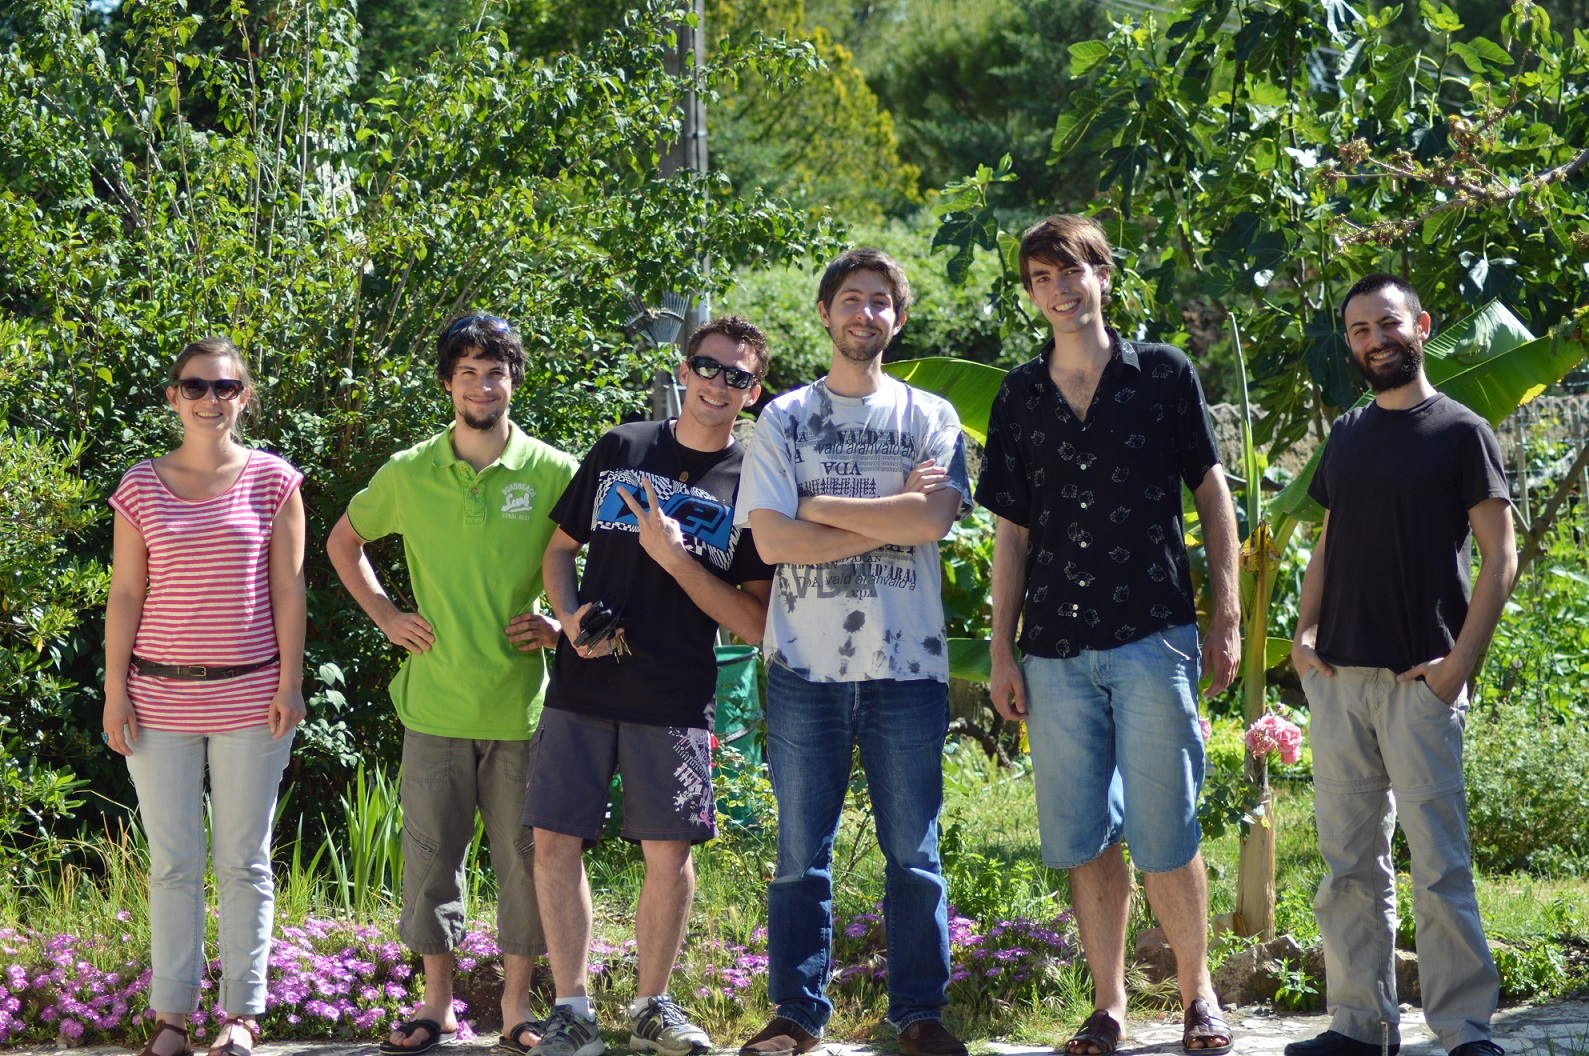
\includegraphics[width=420px]{images/naturalpad_groupe.jpg}
		\caption{Une partie de l'équipe de NaturalPad à Prades le Lez}
		\label{naturalpad_groupe}
	\end{figure}
	
		\subsubsection*{Antoine SEILLES - Fondateur, CEO}
\begin{minipage}[t!]{0.2\linewidth}
\centering

\includegraphics[width=0.8\textwidth]{images/tetocarre/antoine}
\end{minipage}
\begin{minipage}[t!]{0.79\linewidth}
Antoine Seilles est docteur en informatique. Sa thèse, soutenue en avril 2012 porte sur les usages du Web 3.0 (ou web socio-sémantique) dans le contexte de la démocratie électronique. Les domaines de recherche d’Antoine portent essentiellement sur l’aspect social du Web, thème sur lequel il a participé à plusieurs conférences grand public, et sur le Web sémantique, thème sur lequel il a publié à plusieurs reprises et traduit le livre de Tom Heath et Christian Bizer «Linked Data».
		\begin{quotation} \emph{Au sein de NaturalPad} \end{quotation}
Chez NaturalPad, la recherche d’Antoine porte sur les solutions Web 2.0 autour du Dossier Médical Personnel et sur les formats de données utilisant les technologies du Web sémantique (RDF notamment) pour la télémédecine.
\end{minipage}

		\subsubsection*{Sébastien ANDARY - Fondateur}
\begin{minipage}[t!]{0.2\linewidth}
\centering

\includegraphics[width=0.8\textwidth]{images/tetocarre/seb}
\end{minipage}
\begin{minipage}[t!]{0.79\linewidth}
Il a reçu le diplôme de Master d’Informatique à l’Université de Montpellier et termine actuellement un Doctorat de Robotique au LIRMM. Sa thèse porte sur la commande des systèmes mécaniques sous-actionnés dans le cadre de la robotique humanoïde. 
		\begin{quotation} \emph{Au sein de NaturalPad} \end{quotation}
Sébastien travaille au développement de technologies et outils innovants pour la captation de mouvements.
\end{minipage}

		\subsubsection*{Inès DI LORETO - Fondatrice}
\begin{minipage}[t!]{0.2\linewidth}
\centering

\includegraphics[width=0.8\textwidth]{images/tetocarre/ines}
\end{minipage}
\begin{minipage}[t!]{0.79\linewidth}
Elle est diplômée en philosophie et a obtenu un doctorat en informatique à l’Università degli Studi di Milano (Italie). Fin 2009, elle rejoint en postdoc le projet \href{http://www.mojos.fr}{MoJOS}. Dans ce projet de recherche sur les jeux thérapeutiques elle a mené des activités scientifiques pour relever les défis de l’acceptation des patients et des thérapeutes du jeu comme moyen de rééducation. 
		\begin{quotation} \emph{Au sein de NaturalPad} \end{quotation}
Inès travaille sur la transformation des objectifs thérapeutiques en objectifs de jeu en collaboration directe avec les professionnels de la santé.
\end{minipage}

		\subsubsection*{Tristan LE GRANCHE - Fondateur}
\begin{minipage}[t!]{0.2\linewidth}
\centering

\includegraphics[width=0.8\textwidth]{images/tetocarre/tristan}
\end{minipage}
\begin{minipage}[t!]{0.79\linewidth}
Travaillant dans le monde du cinéma d’animation depuis plus de 4 ans, il a travaillé sur plus d’une dizaine de projets de séries télévisées, et de longs et courts métrages. Aujourd’hui il s’est spécialisé dans les Effets Spéciaux Numériques et travaille à l’international en tant que Directeur Technique.
		\begin{quotation} \emph{Au sein de NaturalPad} \end{quotation}
Tristan occupe le poste de Directeur Artistique.
\end{minipage}
	
		\subsubsection*{Benoit LANGE - Fondateur}
\begin{minipage}[t!]{0.2\linewidth}
\centering

\includegraphics[width=0.8\textwidth]{images/tetocarre/ben}
\end{minipage}
\begin{minipage}[t!]{0.79\linewidth}
Il est diplômé d’un master informatique spécialisé en Web et Intelligence Artificielle. Il a ensuite obtenu son diplôme de docteur en informatique à l’université Montpellier 2 en Novembre 2012. Ce doctorat avait pour sujet de réaliser une méthode de visualisation de données afin de permettre l’optimisation énergétique pour le bâtiment. 
		\begin{quotation} \emph{Au sein de NaturalPad} \end{quotation}
Benoit propose, étudie et met en oeuvre des prototypes d’interactions adaptés à des thérapies.
\end{minipage}

		\subsubsection*{Anthony BARREAU - Employé}
\begin{minipage}[t!]{0.2\linewidth}
\centering

\includegraphics[width=0.8\textwidth]{images/tetocarre/anthony}
\end{minipage}
\begin{minipage}[t!]{0.79\linewidth}
Il est diplômé d’une licence professionnelle en informatique spécialité web et gestion. Il a ensuite débuté son expérience professionnelle au sein de l’équipe SMILE du LIRMM. Il a rejoint l’équipe pour participer au développement du projet \href{http://www.mojos.fr}{MoJOS}. Dans ce projet de recherche sur les jeux thérapeutiques, il a participé au développement de prototypes de jeux et d’agents intelligents servant à adapter la difficulté. 
		\begin{quotation} \emph{Au sein de NaturalPad} \end{quotation}
Anthony participe au prototypage et au développement des outils innovants de l’entreprise.
\end{minipage}

		\subsubsection*{Marion FLORIS - Employée}
\begin{minipage}[t!]{0.2\linewidth}
\centering

\includegraphics[width=0.8\textwidth]{images/tetocarre/marion}
\end{minipage}
\begin{minipage}[t!]{0.79\linewidth}
Titulaire d’un D.U.T. Information-Communication et d’une Licence Professionnelle Management des Ressources Numériques, Marion est issue d ’une formation littéraire. Après avoir été libraire spécialisée en bande dessinée pendant deux ans, elle a développé son expertise en Community Management par une formation de 6 mois chez Objectif3D.
		\begin{quotation} \emph{Au sein de NaturalPad} \end{quotation}
Marion est Community Manager et est chargée de la communication.
\end{minipage}

		\subsubsection*{William DYCE - Stagiaire}
\begin{minipage}[t!]{0.2\linewidth}
\centering

\includegraphics[width=0.8\textwidth]{images/tetocarre/william}
\end{minipage}
\begin{minipage}[t!]{0.79\linewidth}
William effectue son stage de Master 2 IMAGINA en même temps que moi chez NaturalPad. L'objectif de son stage était de permettre une reconnaissance des joueurs et de leurs mouvements plus fine avec la Kinect. L'utilisation du Kinect dans un contexte thérapeutique exige en effet une reconnaissance avec des contraintes plus poussées que pour une utilisation purement ludique. Grâce à cela, il sera possible d’imaginer de nouveaux gameplay de jeux basés sur le mouvement.
\end{minipage}

		\subsubsection*{Andy CAMICCI - Stagiaire}
\begin{minipage}[t!]{0.2\linewidth}
\centering

\includegraphics[width=0.8\textwidth]{images/tetocarre/andy}
\end{minipage}
\begin{minipage}[t!]{0.79\linewidth}
Étudiant en licence professionnelle Activité et Techniques de Communication à Arles, Andy a effectué un stage de trois mois de Avril à Juin durant lesquels il a participé au développement de l'interface web thérapeutique et aux modules de visualisation des données de jeux. Nous avons travaillé conjointement afin de fournir un outil ergonomique et efficace pour la paramétrisation des parties des jeux thérapeutiques présents sur la plateforme.
\end{minipage}
		
		\subsubsection*{Kevin BRADSHAW- Stagiaire}
\begin{minipage}[t!]{0.2\linewidth}
\centering

\includegraphics[width=0.8\textwidth]{images/tetocarre/kevin}
\end{minipage}
\begin{minipage}[t!]{0.79\linewidth}
Actuellement en stage, Kevin est en licence Informatique et souhaite devenir developpeur de jeux vidéo. Durant son stage, il concoit et développe son propre jeu de manière indépendante : Zether. Pour cela, il crée les assets graphiques, le son et les diverses fonctionnalités du jeu. \\
Ce jeu a pour dessein de venir se greffer sur la plateforme web de NaturalPad. Kevin a en effet imaginé un gameplay jouable à la fois avec souris+clavier et par les mouvements du corps avec une caméra Kinect. Utilisant une approche différente de la mienne, l'objectif thérapeutique n'est pas clairement défini bien que pris en compte. La plateforme de NaturalPad veut aussi pouvoir accueilir des jeux qui ne sont initialement pas développés dans une optique de rééducation mais dont une telle utilisation est possible.
\end{minipage}
		
		\subsubsection*{Célia GIRONNET - Stagiaire}
\begin{minipage}[t!]{0.2\linewidth}
\centering

\includegraphics[width=0.8\textwidth]{images/tetocarre/celia}
\end{minipage}
\begin{minipage}[t!]{0.79\linewidth}
Stagiaire infographiste, cette étudiante de SupInfoGame contribue à enrichir le monde de Hammer \& Planks en réalisant les modèles 2D et 3D des personnages, monstres et autres décors de cet univers de pirates !
\end{minipage}

	\subsection{Hammer \& Planks}
Hammer \& Planks est le premier jeu sérieux pour la santé de NaturalPad. Il a été conçu en collaboration avec une ergothérapeute, Anaïs Ivorra, dans le but de permettre aux personnes hémiplégiques de retrouver leur faculté d’équilibre. Il a été présenté à diverses occasions lors de salons, qu’ils soient grand public comme le MIG ou spécialisés (\href{http://www.ted.com/tedx/events/5188}{TEDx Montpellier} / \href{http://www.e-virtuoses.net/}{e-virtuoses}). Il a par ailleurs été primé aux e-virtuoses 2013 de Valenciennes dans la catégorie "Serious Game Healthcare" et est largement cité dans un article composé d'une vidéo sur les Serious Game thérapeutiques sur le \href{http://videos.doctissimo.fr/sante/recherche/serious-game-therapeutique.html}{site de doctissimo}.
		
\begin{figure}[htbp]
	\begin{minipage}[c]{.45\linewidth}
		\begin{center}
			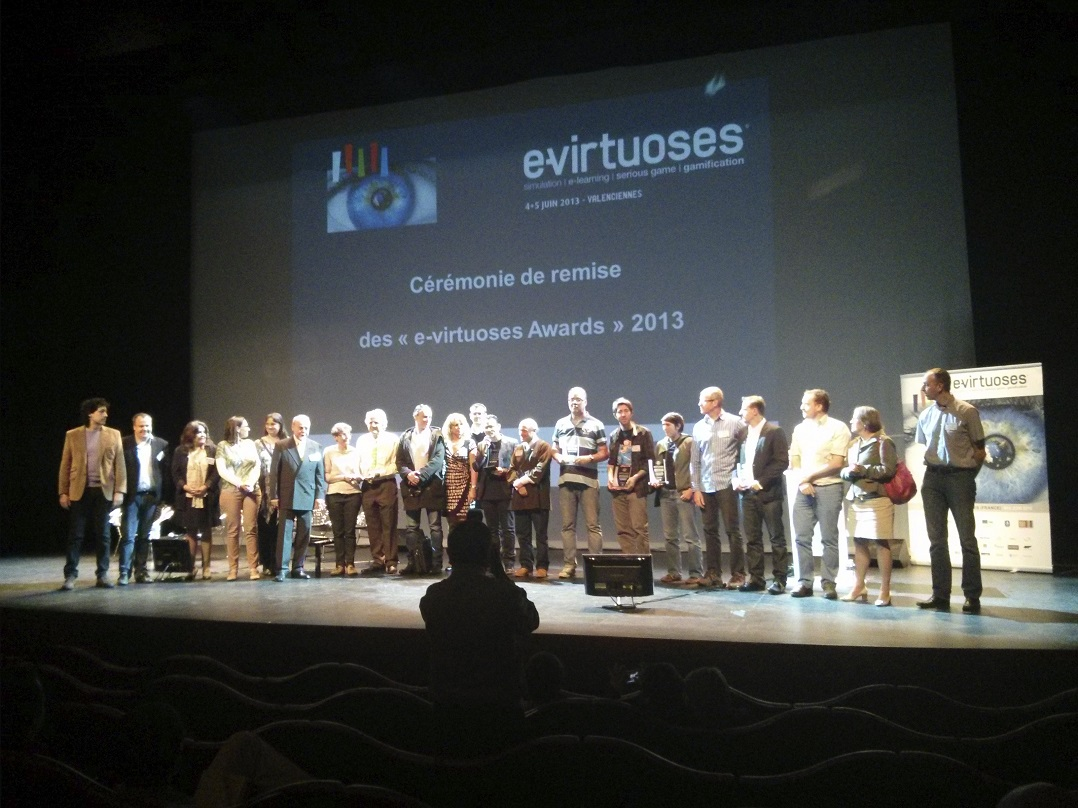
\includegraphics[width=210px, height=157px]{images/remise_awards_e-virtuoses_groupe.jpg}
			\caption{Gagnants des e-virtuoses 2013 dans les différentes catégories.}
			\label{Gagnants}
		\end{center}
	\end{minipage}
	\hfill
	\begin{minipage}[c]{.45\linewidth}
		\begin{center}
			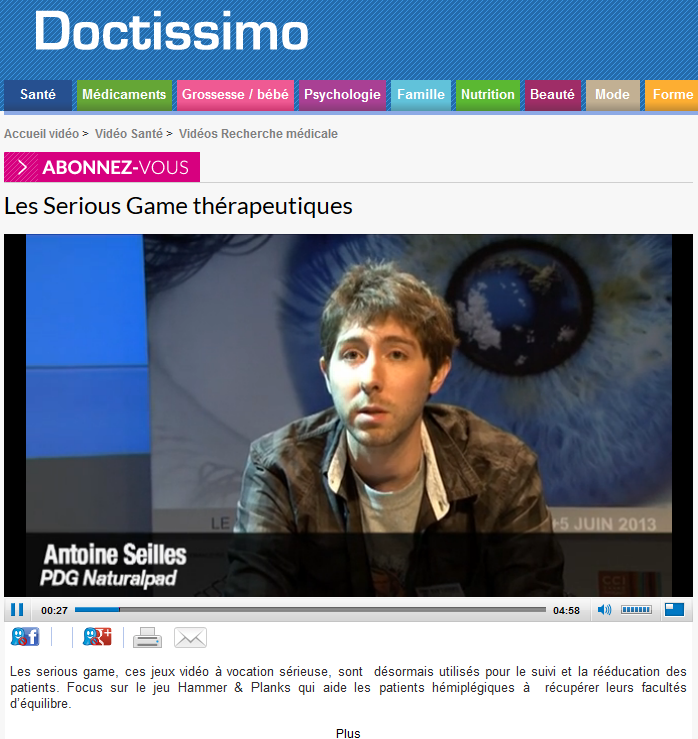
\includegraphics[height=157px]{images/doctissimo.png}
			\caption{Article de doctissimo sur les Serious game thérapeutiques.}
			\label{naturalpad_groupe}
		\end{center}
	\end{minipage}
\end{figure}		

Hammer \& Planks est constitué d’un environnement 3D vu de dessus. Le joueur contrôle un bateau qu'il peut déplacer de gauche à droite et de haut en bas, et peut éliminer les ennemis grâce à ses canons. Enfin, il doit éviter des obstacles et peut récupérer des bonus. Pour contrôler le bateau, il existe plusieurs solutions : on peut utiliser la Kinect, la Wii Board, une manette ou bien le clavier et la souris. Le jeu a initialement été conçu pour une utilisation avec la Wii Board afin de travailler les facultés d'équilibre, que ce soit assis ou debout. Le jeu possède par ailleurs un ensemble de paramètres qui peuvent être paramétrés ou changés en cours de partie, rendant ainsi le jeu devient ajustable selon les besoins thérapeutiques. On notera qu'il existe une version grand public du jeu, où la paramétrisation avancée est remplacée par un enrichissement du gameplay et du scénario notamment.
	\begin{figure}[!t]
		\centering
		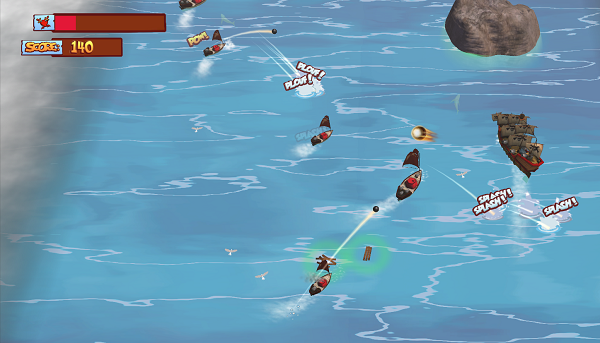
\includegraphics[width=420px]{images/hammer_and_planks.png}
		\caption{Impression d'écran du jeu Hammer \& Planks}
		A droite, le bateau contrôlé par le joueur.
		\label{hammer_and_planks}
	\end{figure}

	
	\newpage
	\section{Problématique}
	\subsection{Sujet et objectifs initiaux}
	Dans ce stage, nous allons nous intéresser à l’adaptation de la difficulté dans un jeu à but thérapeutique sous contrôle d’un médecin. Les variables permettant d’ajuster la difficulté d’un jeu sont nombreuses et variées. Elles peuvent être facilement modifiées et combinées pour créer des objectifs de jeu. Cependant, ces objectifs de jeu n’ont pas nécessairement un sens pour le médecin. Il s’agira dans ce stage de définir avec un thérapeute les variables ou paramètres adaptées à l’adaptation de la difficulté pour le soignant.
	\paragraph{}
	Dans le cadre de ce stage, le stagiaire aura pour mission de:
	\begin{itemize}
		\item {récupérer auprès d’un soignant une liste exhaustive d’objectifs de jeu thérapeutique}
		\item {traduire ces objectifs en paramètres dans le jeu Hammer \& Planks}
		\item {proposer une solution pour suivre et analyser visuellement les progrès du patient relativement aux objectifs fixés par le soignant}
	\end{itemize}
	Le stagiaire devra participer à des séances de coconception avec un thérapeute et sera amené à se déplacer pour suivre des séances de tests auprès de patients.
		
\subsection{Contexte et besoins}
Lors de mon arrivée au sein de NaturalPad, il existant déjà une version du jeu Hammer \& Planks, outil dans lequel devait s'insérer mon travail. Présenté lors du MIG 2012, le jeu était encore surtout orienté grand public. Ma première mission fut donc de m'approprier l'application et de l'adapter pour une utilisation paramétrable dans un contexte thérapeutique. En effet, une utilisation thérapeutique implique d'ajuster les différents paramètres en fonction des capacités et des besoins du patient.

	\paragraph{}Les échanges avec les professionnels de la santé ont été au coeur de mon stage. La compréhension des besoins et des contraintes médicales étant primordiales pour proposer un produit adapté, je me suis naturellement tourné vers les thérapeutes et soignants pour acquérir les connaissances et le background qu'il me manquait. Il m'est par ailleurs rapidement apparu qu'on ne pouvait répondre aux différents besoins thérapeutiques explicités par les soignants avec un seul jeu vidéo, même paramétrable. C'est pourquoi je me suis aussi concentré sur l'aspect de conception avec les thérapeutes. 

	\paragraph{Orientation du travail de stage \\}
Rappelons que la société NaturalPad propose comme outil une plateforme web permettant d'accéder à des jeux sérieux, et de les paramétrer directement depuis celle-ci. Hammer \& Planks constitue ainsi le premier jeu accessible depuis cette plateforme et, bien que servant d'exemple des possibilités d'un jeu vidéo pour la santé, il est amené à être rejoint par d'autres serious games. C'est dans cette optique que mon travail durant ce stage s'est progressivement orienté vers une méthode de conception de serious games pour la santé. Cela a pour objectif de proposer une solution appropriée aux différents besoins et contraintes de chaque situation. Ces derniers peuvent correspondre aux objectifs thérapeutiques, à la pathologie du patient, ses capacités, son âge, sa maitrise des nouvelles technologies ou son aisance avec les jeux vidéo par exemple.
Ce travail s'inscrit donc toujours dans le but d'adapter le jeu vidéo aux besoins thérapeutiques, et est complémentaire à une adaptation des paramètres de jeux, qu'elle soit manuelle ou automatique.
 
\paragraph{}Pour cela, je redéfinirais le sujet de ce stage comme suit :\\
\textcolor{marron}{\emph{ {\large Proposition d'une méthodologie de conception de jeux vidéo sérieux à but thérapeutique, et adaptation de la difficulté.}}}

\subsection{Outils et méthodologie}
	\subsubsection{Méthodologie}
Afin de mener à bien ses projets, l’équipe de NaturalPad emploie une méthode Agile de gestion de projet : SCRUM.

	\paragraph{\emph{Méthodes AGILES}\\}
Les méthodes Agiles sont des groupes de pratiques, réunies dans l'\emph{Agile Manifesto}\cite{Agil01}, s'appliquant dans la gestion de projets, généralement informatiques. Ces méthodes se veulent plus pragmatiques que les méthodes traditionnelles et diffèrent de celles-ci en se concentrant sur des valeurs humaines plutôt que sur les processus. Ce sont des méthodes itératives (ou plutôt semi-itératives), incrémentales et adaptatives.
\begin{figure}
	\centering
	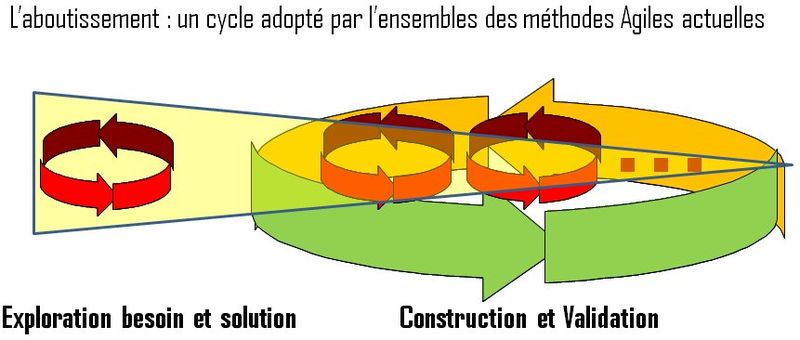
\includegraphics[scale=0.5]{images/agile.jpg}
	\caption{Les méthodes agiles : un cycle semi-itératif}
	\label{agile}
\end{figure}
 
\paragraph{}
Les méthodes agiles prônent 4 valeurs fondamentales :
	\begin{enumerate}
		\item l'équipe : « Les individus et leurs interactions, plus que les processus et les outils. »
		\item L'application : « Des logiciels opérationnels, plus qu'une documentation exhaustive. »
		\item  La collaboration : « La collaboration avec les clients, plus que la négociation contractuelle. »
		\item L'acceptation du changement : « L'adaptation au changement, plus que le suivi d'un plan. »
	\end{enumerate}

		\paragraph{\emph{La méthode Scrum}\\}
Celle-ci définit 3 rôles :
	\begin{itemize}
		\item Le Product Owner
		\item Le Scrum Master
		\item Le Développeur
	\end {itemize}
Le Product Owner est le représentant des clients et des utilisateurs. Son objectif est de maximiser la valeur du produit développé. Il a pour rôle de rédiger des User Stories (comparables à des cas d'utilisation) et de valider le travail des développeurs. 
\\Le ScrumMaster est le responsable de la méthode. Il doit s’assurer qu’elle est correctement mise en application et comprise par les développeurs. Il organise le «Daily Scrum» (voir définition plus bas).
\\Enfin, le Développeur, représente en fait une équipe pluridisciplinaire et auto-organisée : toutes les décisions sont prises ensemble, sans hiérarchie externe ni interne.
 
		\paragraph{Daily Scrum :}
Il s’agit d’une réunion quotidienne ayant pour but de faire un point sur la coordination entre les tâches et les difficultés rencontrées.  Trois questions sont posées aux développeurs : 
	\begin{itemize}
		\item Qu’as-tu fait hier ?
		\item Qu’est-ce que tu vas faire aujourd’hui ?
		\item Est-ce que tu as rencontré des difficultés ?
	\end {itemize}
	
\paragraph{}Le travail est organisé sous forme de sprint. Il s’agit d’une courte période (au maximum un mois) au bout de laquelle l’équipe doit fournir une version améliorée du produit. Chaque sprint possède un but (ex : «on doit pouvoir envoyer des paramètres au jeu») et une liste de tâches (ex : «déterminer la méthode de communication, etc...»). Dès la fin d’un sprint, un nouveau est lancé.

\paragraph{}Enfin, une réunion a lieu en fin de sprint pour faire le point sur le travail accompli, les erreurs rencontrées et comment ne pas les éviter à l'avenir, ainsi que lancer le sprint suivant. Cette méthode est très intéressante car elle permet vraiment de garder une cohésion dans l’équipe de développement et d’avancer de manière visible. 

	\subsubsection{Outils}
		\paragraph{Gestion de projet\\}
Lors de mon arrivée dans l'entreprise, l’équipe utilisait Redmine, une application web de gestion de projets. Nous avons cependant changé deux fois d'outils de gestion de projet pendant la période de ce stage. Le premier est intervenu car les mises à jour des tâches dans Redmine étaient longues et l'outil finalement peu approprié à une méthodologie AGILE, ce qui freinait son utilisation. Nous avons donc mis en place une méthode Kanban qui consiste à écrire chaque tâche sur un post-it, et de déplacer ce post-it dans des colonnes «A faire», «En cours», «Terminé» ou «Validé» selon son avancement par exemple. De cette manière, l’avancement global était bien plus visible mais cette solution était finalement gourmande en post-it et en place. C'est pourquoi, nous utilisons désormais \href{www.trello.com}{Trello}, un outil de gestion de projet en ligne, se basant sur la méthode Kanban. Il s’agit d’un tableau virtuel dans lequel nous pouvons facilement déplacer les tâches, ajouter des commentaires ou des contraintes de temps notamment.

	\begin{figure}[!h]
		\centering
		
\includegraphics[height=48px]{images/redmine.jpg}
		
\includegraphics[height=48px]{images/trello.jpg}
		\caption{Logos de Redmine et Trello}
		\label{logos_redmine_trello}
	\end{figure}
 \newpage
		\paragraph{Développement}
		\subparagraph{} \emph{Unity3D\\}
La majeure partie technique de mon travail a été réalisée pour Hammer \& Planks, qui est développé avec le moteur de jeu Unity3D. Au fil de mon stage, nous sommes passés de la version 3.9 à la version 4.1. Unity permet de facilement intégrer les modèles 3D des objets réalisés dans les logiciels de modélisation 3D tels que Photoshop, Gimp ou Maya. Il propose aussi des options permettant d'utiliser un gestionnaire de versions pour les fichiers du projet.
	\begin{figure}[!h]
		\centering
		
\includegraphics[height=48px]{images/unity.jpg}
		\caption{Logo d'Unity3d}
		\label{logo_unity}
	\end{figure}

		\subparagraph{} \emph{Play! Framework\\}
Play! Framework est un framework open source web qui permet d'écrire rapidement des applications web en Java ou en Scala. Il vise à apporter un outil simple et productif sur la machine virtuelle Java. Play Framework a pour particularité de ne pas être basé sur le moteur Java de Servlet. Il propose par ailleurs un moteur de template basé sur Scala.
	\begin{figure}[!h]
		\centering
		
\includegraphics[height=48px]{images/play.png}
		\caption{Logo de Play! Framework}
		\label{logo_play}
	\end{figure}		

		\subparagraph{} \emph{Git\\}
Que ce soit pour Hammer \& Planks ou nos autres projets en cours, l'utilisation d'un gestionnaire de versions se révèle vite indispensable. Travaillant en équipe allant jusqu'à cinq développeurs et une graphiste, il est nécessaire de pouvoir mutualiser le travail. De plus, l'expérimentation et le développement de nouveaux éléments se prêtent très bien à l'utilisation de plusieurs branches de développement, chose que Git permet de gérer facilement.
	\begin{figure}[!h]
		\centering
		
\includegraphics[height=48px]{images/git.png}
		\caption{Logo de Git}
		\label{logo_git}
	\end{figure}

		\subparagraph{}	\emph{BitBucket et GitHub}
Pour héberger ses projets, NaturalPad avait l'habitude d'utiliser GitHub. Avec l'arrivée de nouveaux stagiaires, il nous a fallu trouver une solution permettant un accès privé au dépôt pour un plus grand nombre de personnes, ce que permet BitBucket.
	\begin{figure}[!h]
		\centering
		
\includegraphics[height=48px]{images/bitbucket.jpg}
		
\includegraphics[height=48px]{images/github.jpg}
		\caption{Logos de BitBucket et Github}
		\label{logos_bitbucket_github}
	\end{figure}

	\subsubsection{Veille}
Le Jeu Vidéo et plus généralement l'Informatique est un domaine en constante évolution dans lequel il est nécessaire de se tenir à jour pour connaître les dernières technologies et actualités. Pour cela, j'ai observé durant l'intégralité de ma période de stage une veille technologique et stratégique. Nouveautés technologiques, logiques ou matérielles, communications d'entreprises ou de salons nationaux et internationaux ou bien encore annonces de sociétés dont le secteur d'activité est compatible avec NaturalPad ont donc été au coeur de mon étude quotidienne.
\paragraph{}Pour faciliter ce travail de veille, par ailleurs inclu dans mon planning, j'utilise un agrégateur de flux RSS, outil indispensable pour gérer aisément un contenu important sur un grand nombre de sources différentes. Il s'agit ensuite de mettre à jour et d'étendre régulièrement les sources en fonction de l'utilité observée de chacune d'entre elle ou des manques ressentis. 
\paragraph{Jeux Vidéo\\ \quad}
Étant étudiant en Informatique, option Image Game and Intelligent Agents, et ayant orienté ma formation vers une spécialité Jeux Vidéo, il m'a semblé important de me tenir à jour en terme d'actualité vidéoludique. J'ai pour cela étendu ma veille aux domaines des jeux vidéo, indépendants ou blockbusters, afin d'en étudier différents aspects tels le business model, le gameplay, les technologies employées ou les mécanismes de jeu innovants par exemple. J'ai ainsi pu testé des technologies récentes comme la console Ouya ou le système de contrôle Leap Motion, qui permet d'interagir en utilisant ses mains et ses doigts. Pour plus d'informations sur le Leap Motion, vous pouvez retrouver mon billet sur le blog de \href{naturalpad.fr/category/naturalblog}{NaturalPad}.
\begin{figure}
	\centering
	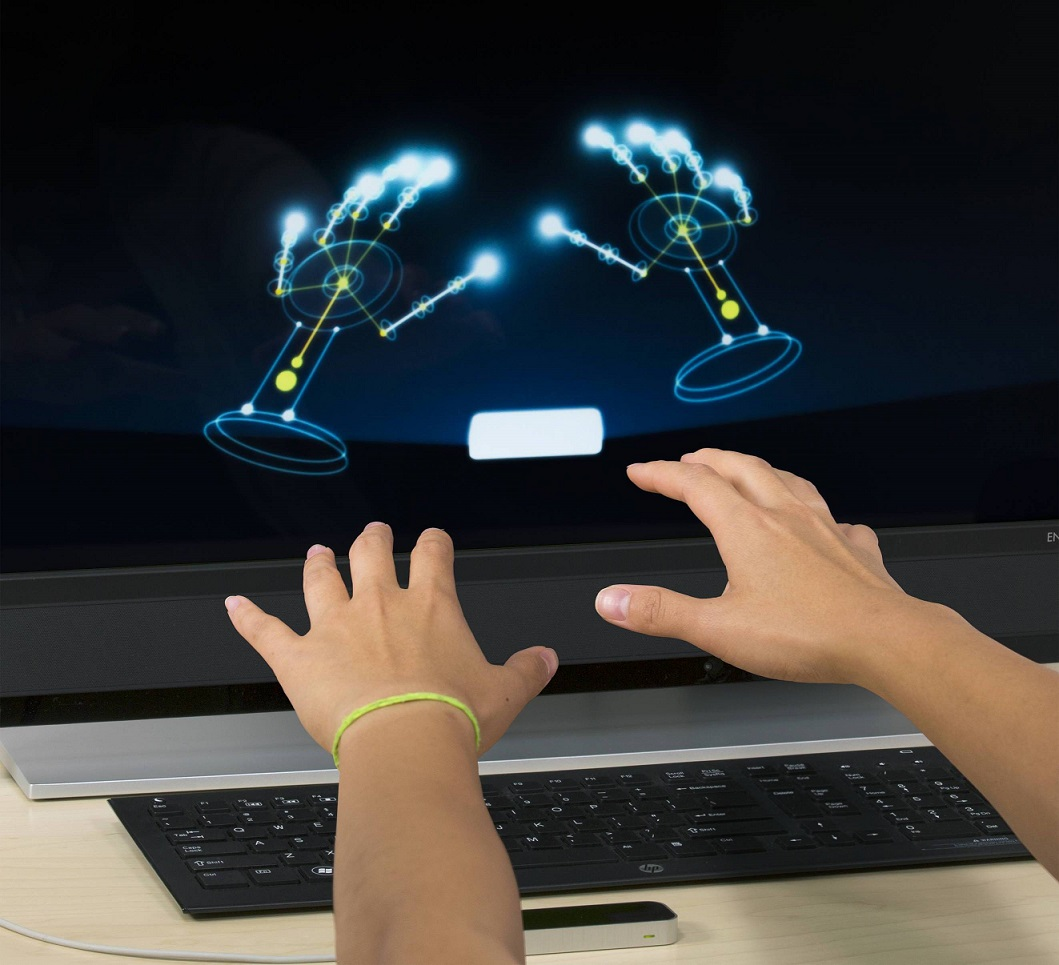
\includegraphics{images/leap_motion.jpg}
	\caption{Utilisation d'un Leap Motion}Une application retranscrit à l'écran la "vision" qu'elle a des mains de l'utilisateur.
	\label{leapmotion}
\end{figure}

	\subsubsection{État de l'art et recherche documentaire}
Étendue sur plusieurs semaines, la réalisation de l'état de l'art était pour moi quelque chose de nouveau qui a nécessité une certaine organisation. Deux moments ont été importants : la phase de démarrage et l'arrêt des recherches. Commencer ces recherches alors que les sujets que je devais ou voulais couvrir étaient vastes et non clairement définis fut à la fois plaisant et compliqué. Bien que beaucoup de choses me semblaient intéressantes, la question était de savoir par où commencer. De la même manière, au fil de mes lectures, je découvrais de nouveaux liens et références présentant de nouveaux aspects qui eux-même renvoyaient vers d'autres solutions et articles. La difficulté était donc de juger quand mes connaissances sur un thème donné étaient suffisantes pour éviter de poursuivre d'interminables recherches, aussi intéressantes puissent elles être, le temps étant limité dans le cadre d'un stage de Master.
	\paragraph{}Au niveau des lectures abordées, ma source principale fut des articles scientifiques, suivie par des articles de magazines spécialisés et articles web notamment. Pour les thèmes médicaux, un certain nombre d'articles m'a été directement conseillé par des professionnels de la santé, articles à partir desquels j'ai ensuite pu compléter mon état de l'art en suivant les références. Par ailleurs, il est fréquent que certains auteurs ressortent régulièrement lorsqu'on effectue des recherches sur un thème donné, ce qui permet, en plus du nombre de citations des articles, de rapidement cerner quels sont les articles et chercheurs de référence dans le domaine.
	\paragraph{}Bien entendu, afin de rendre mes lectures efficaces, je me constituais pour chacune d'elle une fiche de lecture où noter les points importants : 
\begin{itemize}
	\item Titre ou source
	\item Auteur(s)
	\item Mots clefs
	\item Synthèse
	\item Jugement personnel ou remarques
	\item Références importantes
\end{itemize}
	
	\newpage
	\section{État de l'art}
	NaturalPad est une société innovante dont le domaine d'activité est encore à ses débuts. Si les jeux vidéo sérieux commencent à être connus du grand public et leur impact reconnu, ceux pour la santé ne sont pas encore assez nombreux ni assez largement acceptés. Mon travail de stage s'inscrit en réponse à cette constatation : il s'agit de proposer une méthode de conception de jeux vidéo pour la santé qui permettrait une simplification ou une amélioration de la conception de tels jeux. Proposer plus de jeux  thérapeutiques et/ou des jeux avec un impact santé de plus grande qualité contribuerait à améliorer leur diffusion et leur reconnaissance. Pour ces raisons, il était ainsi primordial de parfaire ma connaissance des différents domaines concernés.

Cette partie présente le résultat de mes recherches, des techniques et outils existants et comporte des notions importantes à connaître pour la conception de serious games pour la santé.

	\subsection{Jeux Vidéo}
Durant mon stage, j'ai ainsi voulu comprendre pourquoi et comment un jeu vidéo est bon, quels en sont les mécanismes ou bien encore ce qu'est la difficulté, pourquoi et comment l'adapter.\\

		\subsubsection{Théories cognitives}
Schéma et description.		
		\subsubsection{La difficulté}
Dans son livre \emph{La cigale : jeux, vie et utopie}, le philosophe Bernard SUITS indiquait : \begin{quote}{“Jouer consiste à tenter volontairement de surmonter des obstacles inutiles”}.  \end{quote}
		
			\paragraph{Adaptation de la difficulté\\}
Il est nécessaire d'adapter la difficulté pour chaque joueur pour garantir une expérience de jeu optimale.			
				\subparagraph{personnes âgées\\}
pas/peu d'expérience de jeu, voir même des nouvelles technologies, capacités physiques restreintes, background social à prendre en compte (jeux de cartes préférés aux jeux de guerre) \cite{Csik75}.
				\subparagraph{hémiplégiques\\}		
Contraintes spécifiques.					
			\paragraph{Système de recommandation \\}
(faire de l'adaptation via ce genre de système)
La proposition est ici de s'inspirer du monde la musique (ou libres, films, ventes en ligne) et de son système de recommandation. Il existe en fait deux types de recommandations. La recommandation sociale consiste par exemple à conseiller à un utilisateur des musiques qu'apprécient des personnes de son réseau, notamment si elles écoutent généralement des musiques identiques. Un autre exemple est sur un site de vente en ligne, de proposer à un utilisateur venant d'acheter un objet, une liste d'objets ayant aussi été achetés par d'autres utilisateurs en même temps que le premier objet.
Le second type de recommandation se base pas non pas sur l'environnement social de l'utilisateur, mais sur le contenu même des objets recommandés. L'idée est alors de chercher à décrire un objet selon certaines caractéristiques, et à faire de même pour les préférences de l'utilisateur. On va ensuite lui conseiller les objets qui semblent être le plus proche des attentes de l'utilisateur en se basant sur ces critères de préférences. 
 \paragraph{}
 Dans notre problématique, ce système de recommandation pourrait servir à sélectionner les paramètres de jeux, voir dans de futurs travaux le jeu lui même, qui correspondraient le mieux aux besoins du joueur. Rappelons que ces besoins peuvent être soit explicites, notamment à travers les recommandations et exigences du thérapeute, soit plus inconscients. Ces besoins inconscients représentent pas exemple les préférences du joueur-patient en terme de gameplay. Un jeu plus distrayant et motivant pour le patient renforcera son implication dans le programme de réhabilitation, et donc son rétablissement. Pour cela il faut donc à la fois connaître les préférences du patient, explicites ou `découvertes'  grâce à un système d'apprentissage par exemple, mais aussi s'appuyer sur un certain nombre de théories et connaissances que l'on sait efficaces pour renforcer cette immersion. 		
	\subsection{Les serious games}
Definition et jeux existants.	
		\subsubsection{Serious games pour la santé}
Existence de jeux sérieux à but thérapeutique ayant pour but de faciliter la réhabilitation en maintenant la motivation du patient. Cependant, ces jeux sont encore rares et ne remplissent pas encore parfaitement leur rôle à cause du problème de l'ajustement de la difficulté en fonction du joueur.
Or comme on le verra plus tard, la difficulté joue un rôle important dans la satisfaction et la motivation du joueur. La question se pose donc de savoir comment ajuster de manière dynamique la difficulté d'un jeu afin qu'elle sied au mieux à chaque joueur, à chacune de ses sessions, dans le but final de renforcer la récupération motrice du joueur-patient. On va par ailleurs chercher à fournir le meilleur environnement virtuel possible pour chaque situation, avec ici comme objectif de contexte à terme un couple patient-thérapeute avec considérations des objectifs thérapeutiques. 		
	\subsection{La réhabilitation}
Un autre aspect est la dimension médicale de la rééducation. Connaître les enjeux, les contraintes, le contexte médico-social d'une réhabilitation ainsi que les techniques existantes ou les jeux thérapeutiques existants s'avéraient donc nécessaire.
	
		\subsubsection{Adaptation de la difficulté dans une rééduc fonctionnelle aujourd'hui (exercices de récup sensorielle, de mouvements, etc)}
		
		
	\subsection{Interfaces naturelles (NUI)}
		\subsubsection{Existant}
		
		\subsubsection{Jeux avec NUI (types de jeux)}
		
		
	\subsection{Méthodes de conception}
		\subsubsection{Participative design : conception participative}
		
		\subsubsection{Innovation games}
		
		\subsubsection{Impact mapping}
	
	\newpage
	\section{Proposition}
		-dire ce que je propose et pourquoi (pourquoi et pour quoi/qui, comment ça sera censé être utilisé, dans quel but) :
-> proposition d'une méthode de conception participative de JV thérapeutiques. Préciser les points importants de la conception, comme l'adaptation de la difficulté.
* propositions (théoriques) d'adaptation de de gameplay pour des NUI (m'inspirant de l'existant et des méthodes de rééduc)
	- parler ici de me la phase de veille / test, en testant le leap motion, des jeux sur Wii et Kinect PSMove, me permettant de faire des propositions plus pertinentes sur les controles.
* Cas pratique défini : travail sur l'équilibre (et lombalgie) et devices (kinect et wii)
*définition de la difficulté dans le jeu vidéo thérapeutique (ma position est que c'est différent des jeux classiques)
	
	\newpage
	\section{Réalisation}
	\subsection{Interface thérapeutique pour l'ajustement de la difficulté de serious games}	
\emph{Hammer \& Planks} est, dans sa version thérapeutique, un jeu permettant d'aider à récupérer des facultés motrices dans le cadre d'un accompagnement à la rééducation. Rappelons qu'il s'agit d'un shooter à défilement vertical dans lequel le joueur contrôle un bateau qu'il dirige avec des mouvements du corps. Le joueur doit éviter des obstacles, affronter divers ennemis et ramasser des bonus sur la mer. Tous ces objets possèdent des attributs qu'il est possible de modifier afin d'adapter le jeu aux besoins et aux capacités du patient. Ce fut mon travail durant la première partie de mon stage de permettre de modifier ces paramètres directement à partir d'une interface web contrôlée par le soignant menant la séance de thérapie.
\paragraph{}
Ce projet se divise en deux parties distinctes~:
\begin{enumerate}
	\item L'interface thérapeutique
	\item Le paramétrage des variables de jeu
\end{enumerate}

	\subsubsection*{Interface thérapeutique}
Celle-ci permet, à partir d'un terminal distinct, de choisir un jeu et de lancer une partie sur le terminal utilisé par le patient. Ce dernier sera équipé d'un périphérique de contrôle comme la caméra Kinect ou la wii board. A partir de cette interface, le soignant est en mesure de voir et de modifier l'ensemble des paramètres de jeu (en tout cas, le sous-ensemble considéré comme pertinent et effectivement envoyé à l'application). De plus, à la fin d'une partie, il sera capable de visualiser les données de la session de jeu, comme l'apparition d'évènements ou les zones que le joueur a réussi ou non à atteindre. Ces informations sont utiles pour mieux cibler les difficultés du patient et ajuster au mieux les prochaines séances. Cette partie du projet a été réalisée par Andy Camicci durant son stage chez NaturalPad entre Avril et Juin 2013.

\begin{figure}[htbp]
	\centering
%	\includegraphics[scale=]{images/interface_therapeutique_01.png}
	\caption{TODO Modification des valeurs du jeu dans l'interface thérapeutique}
	\label{interface_therapeutique_01}
\end{figure}

\begin{figure}[htbp]
	\centering
%	\includegraphics[scale=]{images/interface_therapeutique_02.png}
	\caption{TODO Visualisation des données de la partie.}
	\label{interface_therapeutique_02}
\end{figure}

	\subsubsection*{Maitriser la difficulté : le paramétrage des variables de jeu}
Cette partie consiste en l'extraction des paramètres de jeux et en la création d'un système permettant de créer, d'enregistrer et de transmettre des configurations de ces attributs à l'interface thérapeutique.

\paragraph{}
\emph{Hammer \& Planks} est développé avec le moteur de jeu Unity3d et les scripts codés avec le langage de programmation C\#. Comme nous l'avons dit, \emph{H\&P} possède de nombreux contenus contribuant à la richesse du gameplay et aux possibilités d'ajustement. Lors de mon arrivée au sein de NaturalPad, ces objets n'étaient cependant pas ajustables facilement : il fallait rechercher l'ensemble des objets dont on souhaitait modifier un paramètre, trouver les variables correspondant à ces paramètres puis les modifier soit directement dans le code soit par l'intermédiaire de l'éditeur d'Unity. La raison en est que les contraintes de développement du jeu n'ont pas permis de découpler ces informations.

\paragraph{}
Mon premier travail a donc été de découvrir le code et de rechercher toutes les variables dont on souhaiterait potentiellement vouloir modifier la valeur dans un contexte d'ajustement du jeu pour un exercice de rééducation. J'ai ensuite créé une classe spécifique permettant de regrouper conceptuellement les données modifiables. J'ai ainsi regroupé ces données dans des thèmes tels que \emph{réseau}, \emph{ennemis}, \emph{joueur}, \emph{contrôles} ou \emph{cosmétiques}.

\paragraph{}
En parallèle, j'ai aussi procédé au refactoring de l'ensemble des classes possédant ou utilisant un ou plusieurs attributs modifiables. L'intérêt était bien sur d'avoir un accès commun unique à ces valeurs, mais aussi et surtout que les valeurs puissent être modifiées de manière extérieure par l'interface thérapeutique. Par ailleurs, la modification de ces valeurs par l'interface devait être certaine et pérenne, afin que les modifications apportées soit effectivement prises en compte par l'application et donc modifier l'expérience de jeu en direct.

	\subsubsection*{Préparer l'évolution du jeu et de la séance}
Si permettre un ajustement en direct des propriétés du jeu par le soignant était une fonctionnalité que nous voulions impérativement mettre en place, celle-ci peut se révéler contraignante et répétitive si elle est utilisée seule. Nous voulions ainsi la possibilité de pouvoir enregistrer des configurations de paramètres, afin de pouvoir passer de l'une à l'autre aisément sans devoir faire chaque modification séparément. Par ailleurs, cela permet d'envisager beaucoup de possibilités comme la personnalisation de configurations pour des patients, l'adaptation aisée du jeu pour des besoins thérapeutiques différents ou encore l'automatisation d'une progression de la difficulté à l'aide de configuration prédéfinies.

\paragraph{}Afin d'utiliser des fichiers de configurations, il a fallu créer un système permettant de serialiser les données puis de les charger et de les lier à l'instance de jeu.\\
J'ai par ailleurs durant mon stage créer plusieurs fichiers de configuration permettant une évolution progressive de la difficulté dans le mode de jeu Survie de \emph{Hammer \& Planks}, pour sa version grand public.

	\subsubsection{Usage : tests, retours et intégrations}
Si le projet \emph{Hammer \& Planks} a été initié par une étudiante en ergothérapie, il est aussi et surtout développé en collaboration avec le pôle de rééducation du centre hospitalier de Lapeyronie à Montpellier. Comme nous l'avons dit, le projet a évolué et son champs d'action, en plus d'un travail sur l'équilibre, s'étend maintenant à de l'aide à la rééducation des membres supérieurs, du tronc et du bassin. Le travail d'équilibre, qu'il soit debout ou assis, s'effectue en utilisant la balance de la Wii, qui enregistre les changements du centre de gravité du joueur-patient pour contrôler le bateau. L'intégration d'un contrôle avec la Kinect permet au joueur d'utiliser d'autres mouvements de son corps. Il est ainsi possible d'utiliser son bras ou sa main pour diriger le bateau, ou les mouvements du tronc et du bassin que ce soit en position assise ou debout.

\paragraph{} Nous approchant d'une méthode de conception participative, nous avons ainsi réalisé plusieurs séances de tests avec des patients hémiplégiques et leurs thérapeutes. \\
Les premières choses marquantes sont la curiosité et l'enthousiaste général à la fois des patients et du personnel soignant. Peu d'entre eux connaissaient l'existence de jeux sérieux pour la santé, et dans le cas contraire, appréciaient particulièrement l'accent mis sur l'aspect vidéo-ludique de \emph{Hammer \& Planks}. Ce fut donc un premier point très positif pour l'équipe.

\paragraph{} 
Lors de la première séance de tests, nous avons ainsi eu de nombreux retours positifs portant sur la possibilité d'ajuster le jeu en direct, la visualisation des informations de la session de jeu ou encore le plaisir de jeu. Nous avons aussi eu de nombreuses remarques menant à l'ajout de fonctionnalités, notamment par le personnel.\\
Les remarques les plus fréquentes concernaient le visuel du jeu : les soignants craignaient que les graphismes soient trop riches et les effets trop complexes pour des patients hémiplégiques. L'effet visuel des mouvements de la mer fut notamment cité, et la différenciation entre bonus et obstacles (ennemis, projectiles et mines ennemies) jugée trop complexe.\\
Enfin, réaliser des tests pendant une demie-journée nous a aussi permis de juger notre travail de manière différente. Nous avons ainsi remarqué que nous faisions régulièrement voir systématiquement certains ajustements de paramètres, alors que certaines valeurs n'étaient jamais utilisées.

\paragraph{De l'importance des tests utilisateurs\\}Petite anecdote enfin, prouvant définitivement l'importance de réaliser des tests en conditions réelles. Lorsqu'on utilise le jeu avec la Kinect, le joueur doit lever la main afin d'être reconnu comme la personne joueuse parmi les possibles multiples personnes détectées par la caméra. Ce système fonctionnait parfaitement lors de nos test en interne. Or quand une patient hémiplégique a tenté de jouer, le système ne la reconnaissait pas. La raison en était que la patiente avait une hémiplégie du coté gauche et voulait donc jouer avec sa main gauche pour travailler sa rééducation. Or, le système était configuré pour ne détecter qu'une main droite... aucun membre de l'équipe n'étant gaucher, nous n'avions pas détecté ce grossier oubli ! L'erreur a bien sur depuis était corrigée.

	\paragraph{\emph{Intégration}\\}
	Forts de ces retours, nous avons ensuite classé les remarques qui nous été faites et celles que nous avons notées. Puis, nous avons discuté de la pertinence et de l'importance de chacune d'elle, ainsi que des différentes possibilités d'y répondre. \\
	Concernant la surcharge visuelle, pouvant poser des problèmes cognitifs à certains patients, surtout pour des personnes peu voir pas habituées aux jeux vidéo, nous avons mis en place la possibilité d'ajuster les paramètres visuels. Il est possible de modifier le contraste du jeu, la taille des éléments interactifs ou encore de supprimer les objets cosmétiques (requins, mouettes, brouillard, effet de la mer, etc.). Nous avons par ailleurs augmenté la taille des projectiles (ennemis et alliés) et ajouté un effet de trainée, les rendant beaucoup plus visibles.\\
	Concernant les bonus, jugés trop difficiles à ramasser, nous mis en place deux systèmes. Le premier est la possibilité de mettre un halo vert autour des différents bonus, les rendant bien plus visibles. Le second, est un mécanisme d'aimantage des bonus vers le bateau du joueur. Cette attraction, dont le rayon est ajustable dans les settings, permet de récupérer les bonus même si on ne passe pas directement dessus, ce qui est souvent difficile et frustrant pour le joueur.\\
Concernant les paramètres enfin, nous modifié les valeurs par défaut de certains et ajuster les bornes min et max des plages de valeurs.

		
	\paragraph{} Nous avons ensuite réalisé une nouvelle séance de tests du jeu intégrant ces modifications. C'est avec plaisir que nous avons constaté que les réponses apportées étaient pertinentes et plaisaient à nos testeurs. Ce fut aussi l'occasion d'avoir de nouveaux retours et de continuer notre processus de conception participative.
	
\paragraph{montrer un aperçu des valeurs modifiables?} et leur utilité d'un point de vue
ajustement et rééduc. Et peut être aussi des images sur le thème "avant/après" pour montrer l'évolution et l'intéret des test en situation.

	\subsubsection{Conclusion}
	Cette expérience et ce travail sur \emph{Hammer \& Planks} m'ont permis de vérifier l'intérêt et la réelle pertinence de jeux sérieux pour la rééducation. Par ailleurs, l'intégration d'un nouveau périphérique, la Kinect, débloquant de nouveaux gameplay avec un système de jeu identique, m'a confirmé l'importance du moyen de contrôle à la fois sur le gameplay mais aussi et surtout sur la richesse des applications thérapeutiques qui en découle. Enfin, les critiques des soignants et des patients au cours des deux séances de tests m'ont assuré de l'importance et du réel intérêt de pouvoir ajuster manuellement les variables de jeux directement pendant la séance. C'est à la fois très gratifiant pour notre travail et très encourageant pour les possibilités en terme de réhabilitation.
	
\paragraph{}
Cependant, un seul jeu, aussi ajustable soit il, ne peut suffire à répondre à tous les besoins et cas d'utilisation. Il y a trois aspects~:
\begin{enumerate}
	\item le cœur du jeu, qui décrit ses lois, objectifs et règles de fonctionnement. Il est propre au jeu (ou à un type de jeu) et non modifiable.
	\item les variables ajustables, qui ne modifient pas les règles mais définissent entre autres la difficulté.
	\item le gameplay, induit par les deux premiers points ainsi que par les périphériques et méthodes de contrôle utilisés. En général, ces derniers sont pris en compte dès l'établissement du coeur du jeu, certaines associations étant incompatibles.
\end{enumerate}
\paragraph{}
Il est possible de modifier l'expérience de jeu en modifiant la valeur des variables ajustables : c'est ce que nous proposons à l'aide de notre interface thérapeutique. Il est aussi possible d'explorer un gameplay a priori identique avec des contrôleurs différents, rendant ainsi à la fois l'expérience de jeu et les mouvements induits différents.
\\Cependant, même ainsi, un jeu vidéo avec un coregame propre finit par montrer ses limites en terme d'adaptation, et il est alors nécessaire de proposer d'autres types de jeux vidéo si l'on veut explorer de nouvelles pistes de rééducation.\\
Pour cette raison, toujours dans l'idée d'une adaptation de la difficulté, la suite logique était de proposer une méthode permettant d'aider à la conception de jeux sérieux thérapeutiques.

\paragraph{}
\subsection{Conception}
	*conception participative avec Arnaud 
		-impact mapping, carte d'empathie et scénarios d'usage et storyboard
	
	-travail avec les thérapeutes
	-répondre aux objectifs thérapeutique par un gamedesign
		- hammer \& Planks et l'équilibre (voir rapport d'anais)
		- classement des objectifs thérapeutique, carte d'impact
	-ajustement de la difficulté et lien avec la thérapie : impact des paramètres en terme de difficulté (équilibre et dos?)
	
	-proposition de controle naturels pour des jeux pour une utilisation thérapeutiques
	
	\newpage
	\section{Perspectives}
		hammer and planks : (paramètres de difficulté, groupe d'ennemis)\newline
	
	-avoir une information de profil pour cibler la difficulté -> nourrir un systeme de recommandation\\
	-ajustement dynamique de la difficulté selon le profil/résultats du joueur\newline
	-étendre le domaine de la méthodologie à d'autre pathologies et matériels\newline
	-éprouver les propositions de méthodo, sur un cas concret et complet\newline
	-permettre un paramétrage par objectifs non par paramètres permettant de faciliter l'utilisation de la plateforme et des jeux par les thérapeutes \newline
	- Le pb c'est que j'ai rien qui dise clairement "pour tel exercice/objectif, fais plutot ce type de jeu avec tels contrôles. Du coup, est-ce que ca pourrait pas être une forme de perspective? disant que ça nécessiterait du travail et serait moins parfait qu'un truc personnalisé, mais ca permettrait de gagner du temps tout en étant mieux que ce qui existe actuellement

	
	\newpage
	\section{Conclusion}
	Globalement, ce stage était sur le thème des échanges et au carrefour entre le monde informatique et le monde médical. Nous avons vu comment allier l'expérience d'une société dans le développement de jeux vidéo, à la connaissance et l'expertise de professionnels de la santé, pour proposer un jeu sérieux efficace et apprécié des joueurs.

\paragraph{}
Ce stage de fin d'étude fut aussi l'occasion de vérifier sur une période longue de six mois que mon niveau de compétence et mon autonomie de travail étaient suffisants. Si j'avais déjà réalisé un stage de deux mois chez NaturalPad, l'accent avait alors était mis sur le développement et l'acquisition de connaissances web. J'avais à cette époque parlé de mon intérêt pour les échanges avec des professionnels d'autres corps de métier. En ayant reparlé avec Antoine Seilles, nous avons axé mon travail de stage vers de la conception avec des thérapeutes. Cela m'a montré l'importance de la communication dans une équipe et nous a permis de trouver un sujet de stage en accord avec nos besoins et envies respectifs.

\paragraph{}
Durant ce stage, j'ai donc participé au développement du serious game Hammer \& Planks, et ma connaissance du moteur de Unity3d fut un atout. J'ai travaillé aussi bien pour sa version grand public, enrichissant mes compétences en game design, que sur la version thérapeutique d'aide à la rééducation motrice. Celle-ci me permit de tester et mettre en application un système d'ajustement des paramètres du jeu, dans le but d'agir sur la difficulté ou l'adaptation du jeu aux capacités du joueur-patient. Cette adaptation se fait au moyen d'une interface web thérapeutique permettant de modifier la valeurs des variables du jeu ou des paramètres de réglage des contrôles par exemple.

\paragraph{}
Nous avons aussi réalisé des séances de tests avec des thérapeutes et des patients représentant les utilisateurs futurs du jeu. Cela m'a permis de confronter mon travail aux critiques et appréciations de personnes complètement étrangères au travail de développement. Ce fut très constructif à la fois pour mieux comprendre les joueurs, mais aussi d'un point de vue humain. Voir une jeune fille de moins de 20 ans, hémiplégique, et se régalant de jouer à Hammer \& Planks, fut réellement touchant. De la même manière, s'entendre féliciter à plusieurs reprises par un homme de plus de 70 ans en disant que grâce à notre travail il trouvait enfin amusant une activité à l'hôpital, est en soi une récompense.

\paragraph{} C'est d'ailleurs l'aspect positif que je suis venu chercher et trouver en venant travailler chez NaturalPad. Je souhaitais utiliser mes connaissances et compétences informatiques dans un contexte différent que le développement d'applications classiques, et basé sur les échanges humains. NaturalPad est une société dont les valeurs correspondent aux miennes, que ce soit dans les pratiques ou les solutions développées.

\paragraph{} Cela m'amène au point suivant, puisque, comme nous l'avons vu, NaturalPad est une société innovante se positionnant sur le marché des serious games. En correspondance avec ma formation, elle m'a permis d'étendre très largement mes connaissances à ce sujet en m'offrant la possibilité d'effectuer un travail de recherche et d'état de l'art. J'ai ainsi beaucoup appris sur les serious games en général, les théories d'apprentissage ou encore la réhabilitation. Ces recherches me seront particulièrement utiles tout d'abord au niveau des connaissances théoriques acquises, mais aussi au niveau de la démarche de travail effectuée. Je souhaite ainsi poursuivre ce type de travail au moyen d'une thèse, sur les serious games ou la difficulté notamment. 

\paragraph{} J'ai aussi proposé plusieurs outils d'aide à la conception ainsi qu'une méthodologie de conception  de serious games pour la santé. Ces travaux m'ont permis d'explorer différentes pistes, de communiquer avec des chercheurs et des thérapeutes et 
leur proposer ces solutions. De nombreuses perspectives sont possibles pour faire évoluer ces outils ou valider la méthodologie, mais les résultats acquis durant le stage sont prometteurs.

\paragraph{} Durant mon stage, l'équipe de NaturalPad a su me faire confiance en me laissant autonomie, prises de décisions et responsabilités. Après avoir assisté à plusieurs séances de conception participative, Antoine Seilles a jugé que j'étais en mesure de mener ma propre séance en m'invitant à diriger une séance au centre hospitalier d'Alès Cévennes (CHAC). \\
J'ai aussi rencontré de nombreux professionnels de la santé de ma propre initiative, ergothérapeutes ou kinésithérapeutes, en fonction des besoins, contribuant à faire évoluer mon travail dans la bonne direction.

\paragraph{}
Enfin, ce stage fut globalement une très bonne expérience. J'ai beaucoup appris technologiquement grâce aux connaissances et aux partages de mes collègues. J'ai aussi passé six mois de réelle bonne humeur, chacun étant libre de s'exprimer et de proposer.
Dans cette optique, l'équipe a par ailleurs réalisé deux game jam d'une semaine durant la période où j'y ai travaillé. Une game jam consiste en la création d'un jeu sur une période courte. Ce fut l'occasion pour chacun de faire jouer son imagination, de mettre en place ses idées et de changer de contexte de travail d'une manière des plus agréables. Les mini-jeux réalisés nous plaisent d'ailleurs particulièrement, et je recommande à tout fan de jeux vidéo de se lancer dans cette expérience.
	
	\newpage
	\section{Bibliographie et sources}
	\bibliography{rapport}

\newpage
\part{Annexes} \appendix
	\section{Les différents types 'classiques' de Jeux Vidéo}
	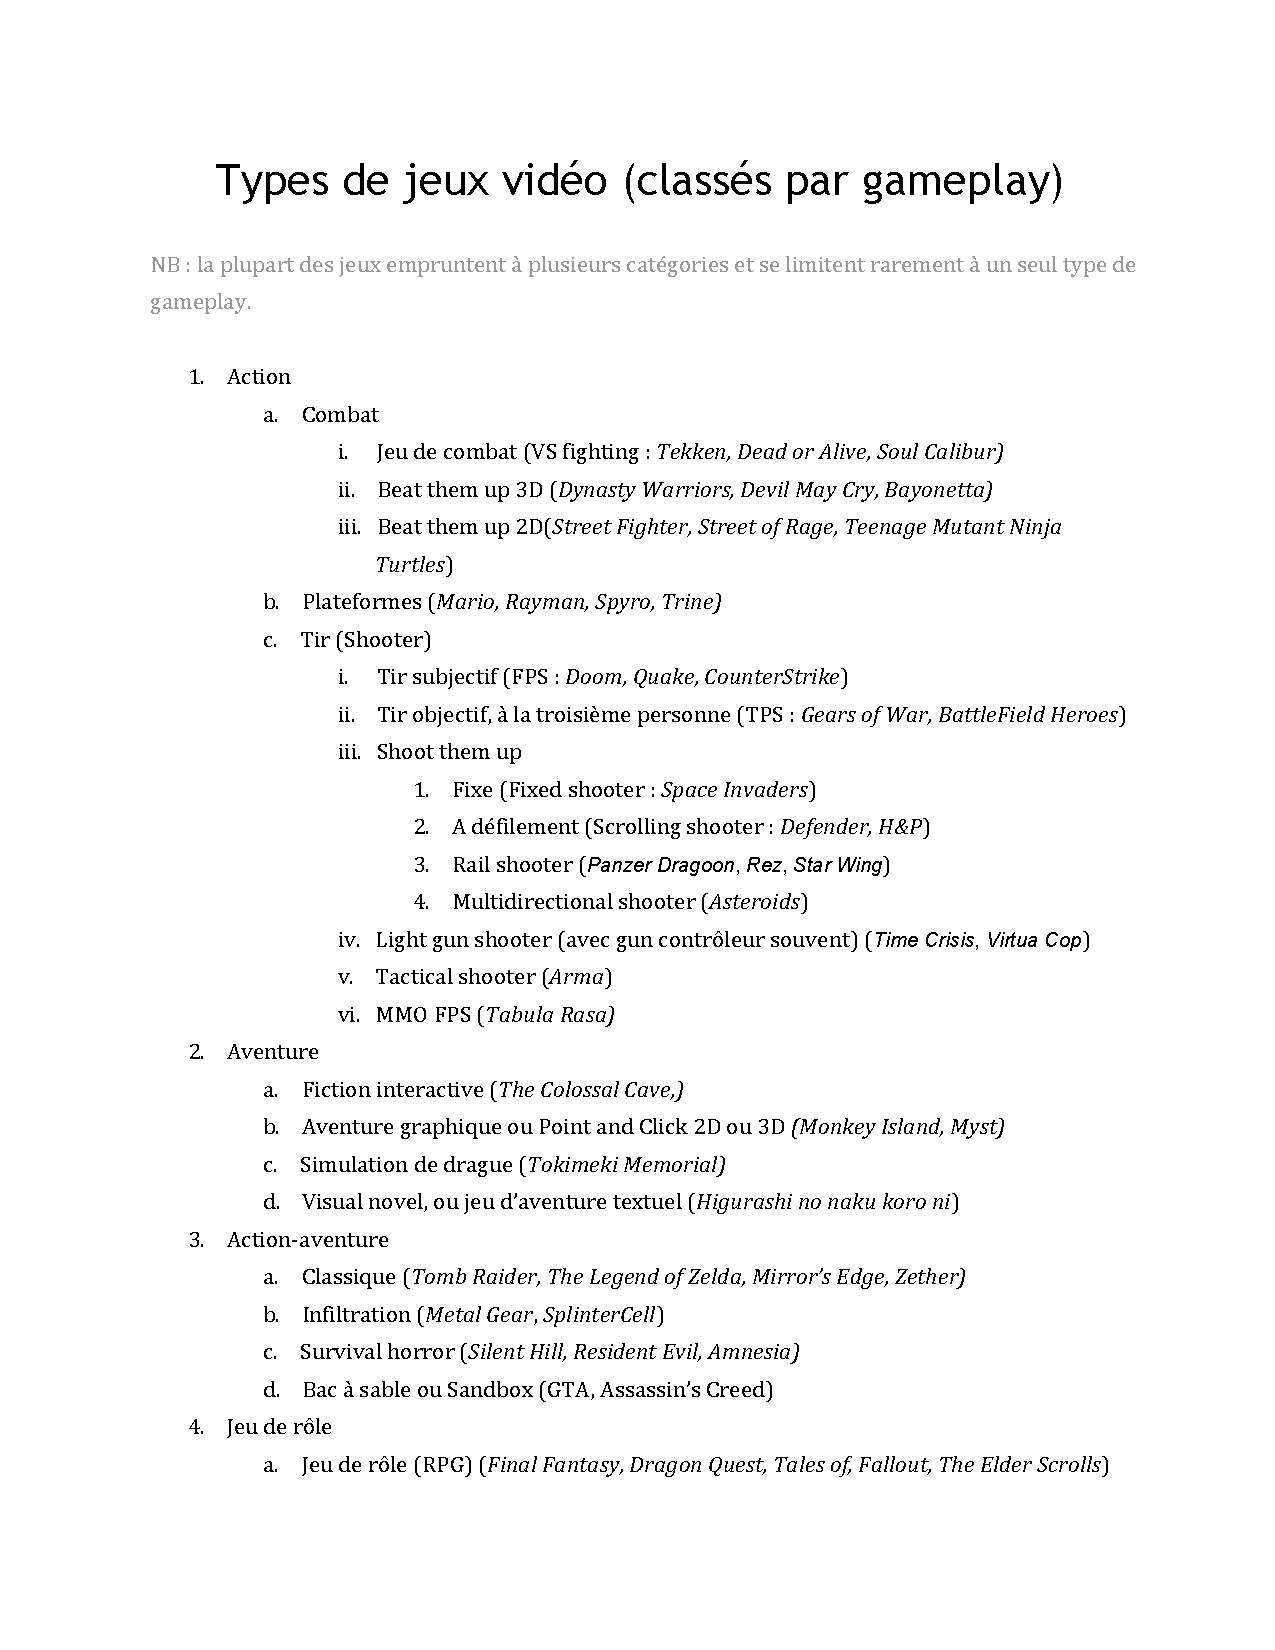
\includepdf[pages=-]{chapters/types_jeux_video} %inclusion de toutes les pages du pdf
	
	\section{Gamejam 1}
	\input{chapters/gamejam_one}
	
	\section{Gamejam 2}
	\input{chapters/gamejam_two}

Voir dans quelle mesure il peut être intéressant de mettre mes comptes rendus d'entretien. Dans des annexes séparées éventuellement.
\end{document}